% arguelles v2.3.0
% author: Michele Piazzai
% contact: michele.piazzai@uc3m.es
% license: MIT

% Copied from GitHub: https://github.com/piazzai/arguelles

\documentclass[compress,12pt]{beamer}

\usetheme{Arguelles}

\title{The Algebra of Logic Tradition}
\subtitle{Proof: A thematic history \#2}
\event{}
\date{}
\author{Navid Rashidian}
\institute{University of Tehran}
%\email{}
%\homepage{}
%\github{}

\newcommand*{\is}{\ \ -\mkern-7mu<}
\newcommand*{\add}{+\mkern-4mu,}

\begin{document}

\frame[plain]{\titlepage}

\Section{Introduction}

\begin{frame}
    \begin{quote}
        The first clear idea of a mathematical logic was formulated by Leibniz. The first results were obtained by A. de Morgan (1806--1876) and G. Boole (1815--1864). The entire later development goes back to Boole. Among his successors, W. S. Jevons (1835--1882) and especially C. S. Peirce (1839--1914) enriched the young science. Ernst Shr\"oder systematically organized and supplemented the various results of his predecessors in his \textup{Vorlesungen \"uber die Algebra der Logik} (1890--1895), which represents a certain completion of the series of developments proceeding from Boole. (Hilbert and Ackermann 1938)
    \end{quote}
\end{frame}

\begin{frame}
    \frametitle{The Algebra of Logic Tradition}
    \begin{itemize}
        \item Augustus De Morgan (1806--1871)
        \item George Boole (1815--1864)
        \item William Stanley Jevons (1835--1882)
        \item Charles Sanders Peirce (1839--1914)
        \item Christine Ladd-Franklin (1847--1930)
        \item Oscar Howard Mitchell (1851--1889)
        \item Ernst Shr\"oder (1841--1902)
        \item Leopold L\"owenheim (1878--1957)
        \item Thoralf Skolem (1887--1963)
    \end{itemize}
\end{frame}

\begin{frame}
    \frametitle{The Advent of Symbolical Algebra}
    \begin{quote}
        The light, then, in which I would consider symbolical algebra, is, that it is
        the science which treats of the combination of operations defined not by their
        nature, that is, by what they are or what they do, but by the laws of combination
        to which they are subject. And as many different kinds of operations may be
        included in a class defined in the manner I have mentioned, whatever can be
        proved of the class generally, is necessarily true of all the operations included
        under it. This, it may be remarked, does not arise from any analogy existing
        in the nature of the operations, which may be totally dissimilar, but merely from
        the fact that they are all subject to the same laws of combination. (Gregory 1840)
    \end{quote}
\end{frame}



\section{Boole's Logic}

\begin{frame}
    \frametitle{George Boole (1815--1864)}
    \begin{columns}
        \begin{column}{0.5\textwidth}
            \begin{center}
                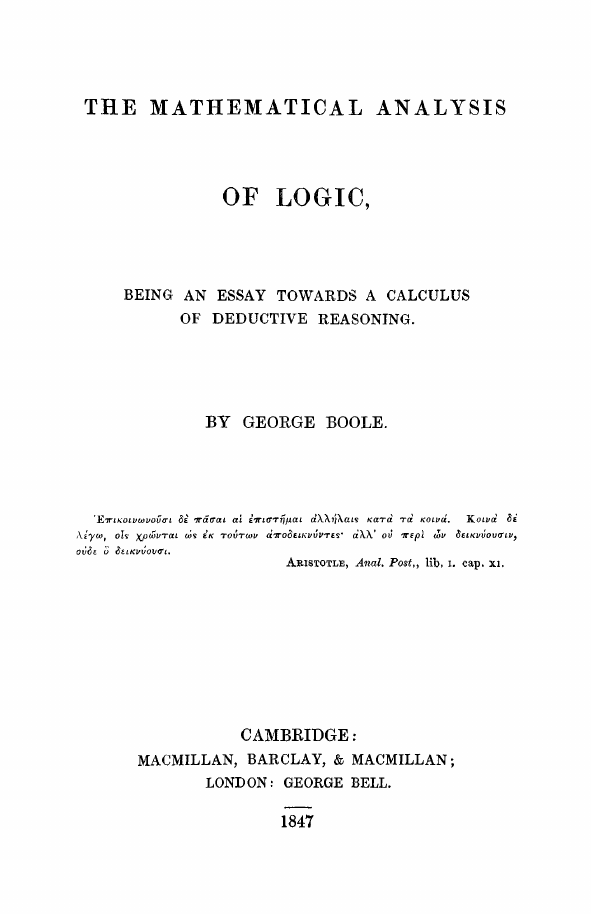
\includegraphics[width=0.8\textwidth]{amal}
            \end{center}
        \end{column}
        \begin{column}{0.5\textwidth}
            \begin{center}
                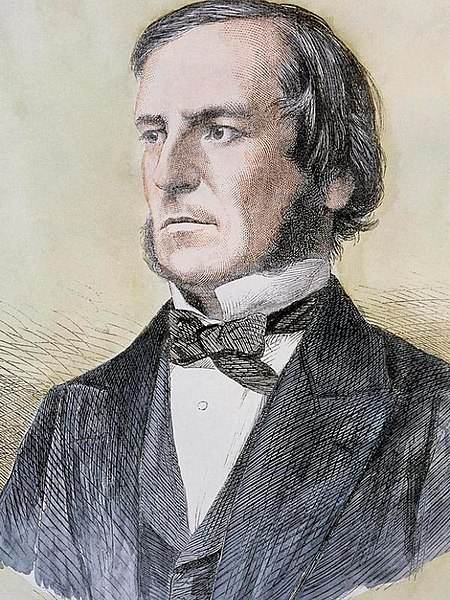
\includegraphics[width=0.8\textwidth]{boole}
            \end{center}
        \end{column}
    \end{columns}
\end{frame}

\begin{frame}
    \frametitle{The Calculus of Logic}
    \begin{quote}
        They who are acquainted with the present state of the theory
        of Symbolical Algebra, are aware, that the validity of the
        processes of analysis does not depend upon the interpretation
        of the symbols which are employed, but solely upon the laws
        of their combination... But the full recognition of the consequences of this important
        doctrine has been, in some measure, retarded by accidental
        circumstances. It has happened in every known form of
        analysis, that the elements to be determined have been con-
        ceived as measurable by comparison with some fixed standard.
        The predominant idea has been that of magnitude, or more
        strictly, of numerical ratio.
    \end{quote}
\end{frame}

\begin{frame}
    \frametitle{The Calculus of Logic (cont'd.)}
    \begin{quote}
        That to the existing forms of Analysis a quantitative interpretation is assigned, is the result of the circumstances by which those forms were determined, and is not to
        be construed into a universal condition of Analysis. It is upon
        the foundation of this general principle, that I purpose to
        establish the Calculus of Logic, and that I claim for it a place
        among the acknowledged forms of Mathematical Analysis, regardless that in its object and in its instruments it must at
        present stand alone. (p. 3--4)
    \end{quote}
\end{frame}

\begin{frame}
    \frametitle{Elective symbols}
    \begin{quote}
        Let us employ the symbol 1, or unity, to represent the
        Universe, and let us understand it as comprehending every
        conceivable class of objects whether actually existing or not,
        it being premised that the same individual may be found in
        more than one class, inasmuch as it may possess more than one
        quality in common with other individuals. Let us employ the
        letters X, Y, Z, to represent the individual members of classes,
        X applying to every member of one class, as members of that
        particular class, and Y to every member of another class as
        members of such class, and so on, according to the received language of treatises on Logic.
    \end{quote}
\end{frame}

\begin{frame}
    \frametitle{Elective symbols (cont'd.)}
    \begin{quote}
        Further let us conceive a class of symbols x, y, z, possessed
        of the following character.
        The symbol $x$ operating upon any subject comprehending
        individuals or classes, shall be supposed to select from that
        subject all the Xs which it contains. In like manner the symbol
        y, operating upon any subject, shall be supposed to select from
        it all individuals of the class Y which are comprised in it, and
        so on. (p. 15)
    \end{quote}
\end{frame}

\begin{frame}
    \frametitle{Laws of combination and succession}
    \begin{quote}
        Our present
        concern is rather with the laws of combination and of succession,
        by which its results are governed, and of these it will suffice to
        notice the following.
        1st. The result of an act of election is independent of the
        grouping or classification of the subject...
        We may express this law mathematically by the equation
        $$x(u+v)=xu+xv$$
        $u + v$ representing the undivided subject, and $u$ and $v$ the
        component parts of it.
    \end{quote}
\end{frame}

\begin{frame}
    \frametitle{Laws of combination and succession (cont'd.)}
    \begin{quote}{\setlength{\abovedisplayskip}{0pt}
        \setlength{\belowdisplayskip}{0pt}
        2nd. It is indifferent in what order two successive acts of
        election are performed.
        The symbolical expression of this law is $$xy=yx\textup{.}$$
        3rd. The result of a given act of abstraction performed twice,
        or any number of times in succession, is the result of the same
        act performed once...
        Thus we have $$xx=x\textup{,}$$
        or \vspace{-5mm}$$x^2=x\textup{;}$$
        and supposing the same operation to be $n$ times performed, we have $$x^n=x\textup{,}$$ which is the mathematical expression of the law above stated. (pp. 16--7)}
    \end{quote}
\end{frame}

\begin{frame}
    \frametitle{Expressing propositions}
    \begin{quote}
        The primary canonical forms... determined for the
        expression of Propositions, are
        \begin{center}
        \begin{tabular}{l r l}
            All Xs are Ys, & $x(1-y)=0$ & ....A.\\
            No Xs are Ys, & $xy=0$ & ....E.\\
            Some Xs are Ys, & $v=xy$ & ....I.\\
            No Xs are not Ys, & $v=x(1-y)$ & ....O.
        \end{tabular}
      \end{center}

        (p. 26)
    \end{quote}
\end{frame}

\begin{frame}
    \frametitle{Categorical syllogisms}
    \begin{quote}
        Ex. AE, Fig. 2, and, by mutation of premises, EA, Fig, 2.
        \begin{center}
            \begin{tabular}{l r r}
                All Xs are Ys, & $x(1-y)=0$, & or\ \ \ $x=xy$ \\
                No Zs are Ys, & $zy=0$, & $zy=0$ \\
                & & $zx=0$ \\
                & & $\therefore$ No Zs are Xs.    
            \end{tabular}
        \end{center}
        (p. 35)
    \end{quote}
\end{frame}

\begin{frame}
    \frametitle{Hypothetical syllogisms}
    \begin{quote}
        To the symbols $X$, $Y$, $Z$, representative of Propositions, we
        may appropriate the elective symbols $x$, $y$, $z$, in the following
        sense.
        The hypothetical Universe, $1$, shall comprehend all conceivable cases and conjunctures of circumstances.
        The elective symbol x attached to any subject expressive of
        such cases shall select those cases in which the Proposition $X$
        is true, and similarly for $Y$ and $Z$. (p. 49)
    \end{quote}
\end{frame}

\begin{frame}
    \frametitle{Translating disjunctive propositions}
    \begin{quote}
        RULE. \textup{Consider what are those distinct and mutually exclusive
        cases of which it is implied in the statement of the given Proposition, that some one of them is true, and equate the sum of their
        elective expressions to unity. This will give the equation of the
        given Proposition.}
        (p. 52)
    \end{quote}
\end{frame}

\begin{frame}
    \frametitle{A hypothetical syllogism}
    \begin{quote}
        Disjunctive Syllogism.

        \begin{tabular}{l c}
            Either X is true, or Y is true (exclusive), & $x+y-2xy=1$\\
            But X is true, & $x=1$ \\
            Therefore Y is not true, & $\therefore\ y=0$           
        \end{tabular}
        (p. 56)
    \end{quote}
\end{frame}

\section{Peirce's Logic}

\begin{frame}
    \frametitle{Charles Sanders Peirce (1839--1914)}

    \begin{columns}
        \begin{column}{0.4\textwidth}
            \begin{center}
                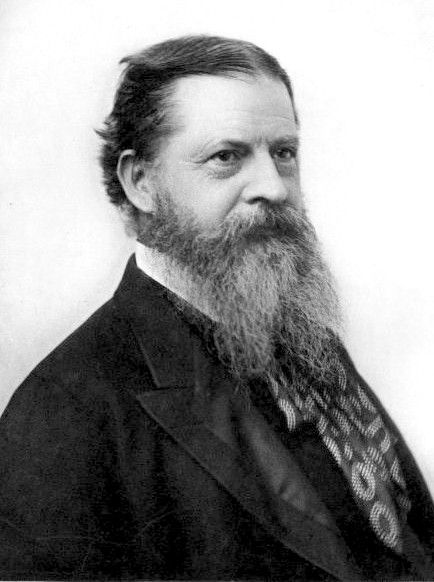
\includegraphics[width=\textwidth]{peirce}
            \end{center}
        \end{column}
        \begin{column}{0.6\textwidth}
            \begin{itemize}
                \item 1870, “Description of a Notation for the Logic of Relatives, Resulting from An Amplification of the Conceptions of Boole’s Calculus” [DNLR]
                \item 1882, “Brief description of the algebra of relatives”
                \item 1883, “The Logic of Relatives”
                \item 1885, “On the Algebra of Logic: A Contribution to the Philosophy of Notation”
            \end{itemize}
        \end{column}
    \end{columns}

\end{frame}

\begin{frame}
    \frametitle{Extending Boole's logical algebra}
    \begin{quote}
        Boole’s logical algebra has such singular beauty, so far as it goes, that it is interesting to inquire whether it cannot be
        extended over the whole realm of formal logic, instead of being
        restricted to that simplest and least useful part of the subject,
        the logic of absolute terms, which, when he wrote, was the only
        formal logic known. The object of this paper is to show that an affirmative answer can be given to this question. (DNLR [CP. 3.45])
    \end{quote}
\end{frame}

\begin{frame}
    \frametitle{Inclusion}
    \begin{quote}
        It will follow from these significations of $=$ and $<$ that the sign $\is$ (or $\leqq$, ``as small as'') will mean ``is.'' Thus,
        $$f\is m$$
        means ``every Frenchman is a man,'' without saying whether there are any other men or not. So,
        $$m\is l$$
        will mean that every mother of anything is a lover of the same thing[.] (DNLR [CP 3.66])
    \end{quote}
\end{frame}

\begin{frame}
    \frametitle{Addition}
    \begin{quote}
        The sign of addition is taken by Boole, so that
        $$x+y$$
        denotes everything denoted by $x$, and, \textup{besides}, everything denoted by $y$... But if there is anything which is denoted by both the terms of the sum, the latter no longer stands for any logical term... For this reason alone... I preferred to take as the regular addition of logic a non-ivertible process, such that
        $$m\add b$$
        stands for all men and black things, without any implication that the black things are to be taken besides the men[.] (DNLR, [CP 3.67])
    \end{quote}
\end{frame}



\begin{frame}
    \frametitle{Multiplication}
    \begin{quote}{\setlength{\abovedisplayskip}{0pt}
        \setlength{\belowdisplayskip}{0pt}
        I shall adopt for the conception of multiplication \textup{the application of a relation}, in such a way that, for example, $lw$ shall denote whatever is lover of a woman... $s(m\add w)$ will, then, denote whatever is servant of anything of the class composed of men and women taken together. So that
        $$s(m\add w)=sm\add sw$$
        $(l\add s)w$ will denote whatever is lover or servant to a woman, and
        $$(l\add s)w=lw\add sw$$
        $(sl)w$ will denote whatever stands to a woman in the relation of servant of a lover, and
        $$(sl)w=s(lw)$$
        Thus all the absolute conditions of multiplication are satisfied. (DNLR, [CP 3.68])}
    \end{quote}
\end{frame}

\begin{frame}
    \frametitle{Involution}
    \begin{quote}{\setlength{\abovedisplayskip}{0pt}
        \setlength{\belowdisplayskip}{0pt}
        I shall take involution in such a sense that $x^y$ will denote everything which is an $x$ for every individual of $y$. Thus $l^w$ will be a lover of every woman. Thus $(s^l)^w$ will denote whatever stands to every woman in the relation of sevant of every lover of hers; and $s^{(lw)}$ will denote whatever is a servant of everything that is lover of a woman. So that
        $$(s^l)^w=s^{(lw)}$$
        (DNLR [CP 3.77])}
    \end{quote}
\end{frame}

\begin{frame}
    \frametitle{Classes as sums of individuals}
    \begin{quote}{\setlength{\abovedisplayskip}{0pt}
        \setlength{\belowdisplayskip}{0pt}
        The fundamental formulae relating to individuality are two. Individuals are denoted by capitals.
        $$\textup{If } x>0\quad x=X\add X'\add X''\add X'''\add\ \textup{etc.}$$
        $$y^X=yX$$
        (DNLR [CP 3.96])}
    \end{quote}\quad
    \begin{quote}
        {\setlength{\abovedisplayskip}{0pt}
            \setlength{\belowdisplayskip}{0pt}
            Let $A$,$B$,$C$,etc., denote objects of any kind. These letters may be conceived to be finite in number or innumerable. The sum of them, each affected by a numerical coefficient (which may equal $0$), is called an \textup{absolute term}. Let $x$ be such a term; then we write
            $$x=(x)_aA+(x)_bB+(x)_cC+\textup{etc.}=\Sigma_i(x)_iI$$
            (1882 [CP 3.306])}
    \end{quote}
\end{frame}

\begin{frame}
    \frametitle{Relatives as classes of pairs of objects}
    \begin{quote}{\setlength{\abovedisplayskip}{0pt}
        \setlength{\belowdisplayskip}{0pt}
        A dual relative term, such as ``lover,'' ``benefactor,'' ``servant,'' is a common name signifying a pair of objects...

        Let $l$ denote ``lover''; then we may write
        $$l=\Sigma_i\Sigma_j(l)_{ij}(I:J)$$
        where $(l)_{ij}$ is a numerical coefficient, whose valuse is $1$ in case $I$ is a lover of $J$, and $0$ in the opposite case, and where the sums are to be taken for all individuals in the universe.
        (1883 [CP 3.328--9])}
    \end{quote}
\end{frame}

\begin{frame}
    \frametitle{Quantifiers, finally!}
    \begin{quote}{\setlength{\abovedisplayskip}{0pt}
        \setlength{\belowdisplayskip}{0pt}
        Any proposition whatever is equivalent to saying that some complexus of aggregates [sums] and products of such numerical coefficients is greater than zero. Thus,
        $$\Sigma_i\Sigma_jl_{ij}>0$$
        means that something is a lover of something; and
        $$\Pi_i\Sigma_jl_{ij}>0$$
        means that everything is a lover of something. We shall, however, naturally omit, in writing the inequality, the ``$>0$'' which terminates them all; and the above two propositions will appear as
        \begin{center}
            $\Sigma_i\Sigma_jl_{ij}$\quad and\quad $\Pi_i\Sigma_jl_{ij}$.
        \end{center}(1883 [CP 3.351])}
    \end{quote}
\end{frame}

\begin{frame}
    \frametitle{A method of derivation}
    \begin{quote}
        I shall, however, content myself here with showing how, when a set of premisses are given, they can be united
        and certain letters eliminated. Of the various methods which
        might be pursued, I shall here give the one which seems to me
        the most useful on the whole. (1885 [CP 3.396])
    \end{quote}
\end{frame}

\End

\begin{frame}[plain, standout]
      \centering\large
      Thank you for your attention!
      
\end{frame}

\end{document}
